\section{Research Methodology}
\label{Methodology}

In this section, an in-depth study will be conducted to solve the challenges outlined in the \nameref{objective}. The section will first discuss the process of dataset selection. Next, several object detection candidates will be analyzed.  The selected object detection method will be examined in multiple domain-adaptive setups. Upon analyzing the existing DA methods, one candidate will be studied in greater detail to propose a novel architecture. Finally, continual learning will be investigated in the selected cross-domain object detection model. 


\subsection{Dataset}
\label{datasets} 
One of the objectives of this thesis was to implement an identification system using images of the equipment and images of the 3D models to expand the dataset. 3D images of the equipment can potentially be the main source of the dataset. Autodesk Navisworks offers a possibility of rendering both images and videos of the desired equipment. In order to make the process of data collection scalable, it was proposed to use Navisworks API to automate the process. Following the documentation of the API  \cite{navisworks}, a simple script with an extra toolbox was used to filter out the required model from Navisworks, to render and to export images in \texttt{.jpg} format. The results are presented in Figure \ref{navisworks} below.

\begin{figure}[htb]
    \centering
    \subfloat{{\includegraphics[width=6cm]{./toolbox.png} }}%
    \qquad
    \subfloat{{\includegraphics[width=6cm]{./model.png} }}%
    \caption{Example of the rendered image of an arbitrary model.}\label{navisworks}%
\end{figure}

It is possible to automatically rotate around the selected object in order to render images from all sides of the equipment as it is important to have variety while accumulating a dataset. However, due to the time constraints, it was decided to leverage existing open-source datasets for the purpose of this study. 

Previously, in the \nameref{neural_nets} section, few datasets, such as ImageNet \cite{Russakovsky2014}, PASCAL VOC \cite{Everingham10} and COCO \cite{Lin2014} were briefly mentioned. These datasets are universally used in image classification and object detection problems. However, in order to leave room for further research as well as to align with the objectives of the thesis, the dataset should ideally consist of industrial equipment and include corresponding 3D models for each object. Datasets such as ImageNet, PASCAL VOC and COCO typically contain generic objects that people face in everyday life. 

Ultimately, it was concluded that the dataset named Texture-LESS (T-LESS)  \cite{hodan2017tless} meets the requirements. It consists of nearly 50 000 training and 10 000 testing images of thirty industry-relevant objects. The training subset consists of rendered images in a simulated environment, while the test subset is taken in real-life conditions.  Different objects in the dataset are often distantly similar to each other, which makes the task slightly more challenging. Finally, the dataset also includes Computer-Aided-Design(CAD) \texttt{.ply} files with 3D models of the objects, which can then be easily converted into any other required CAD format. The dataset is originally meant for 6D-pose estimation \cite{hodan2017tless} as a part of the Benchmark for Pose Estimation(BOP) challenge \cite{hodan2018bop}. As a result, the format of the dataset is derived from the format defined by BOP \cite{hodan2018bop_format}. A script was developed to convert it into a format commonly used by the state-of-the-art object detection frameworks, as well as to remove redundant information that is only applicable to pose estimation tasks. Initially, the dataset was converted to mimic YOLO \cite{Redmon2015a} format, but later it was switched to PASCAL VOC due to its better flexibility in two-stage object detectors. An example of the annotated T-LESS image from a real environment is illustrated in Figure \ref{tless_real_example}. 

\begin{figure}[htb]
	\begin{center}
		\includegraphics[width=10cm]{./tless_real_annotated.png}
	\end{center}
	\caption{T-LESS real setup, labeled
\cite{hodan2017tless}.}
	\begin{center}
		\label{tless_real_example}
	\end{center}
\end{figure}

The names of the object classes presented in T-LESS, although undisclosed, are irrelevant to this thesis. Therefore, here and in the subsequent sections, the classes will be named as "\texttt{Model $N$}", when referred to individually. Additionally, in the experiments, the datasets with images from the simulator and the images from the real environment setup will be mainly referred to as "source" and "target" datasets, respectively. The images from the source dataset are saved in \texttt{.jpg} format, while the real images are stored as \texttt{.png} files, identically as in the original T-LESS \cite{hodan2017tless} dataset. Figure \ref{tless_distribution_rend} illustrates the distribution of the instances by classes in the source dataset.  

\begin{figure}[htb]
	\begin{center}
		\includegraphics[width=14cm]{./rendered_distribution.png}
	\end{center}
	\caption{Distribution of the classes in the rendered subset of T-LESS dataset. Total number of images: 42 500. Total number of object instances: 661598.}
	\begin{center}
		\label{tless_distribution_rend}
	\end{center}
\end{figure}

As can be derived from the \nameref{objective}, the detection accuracy on the source dataset is irrelevant in this thesis. The primary goal is to evaluate the performance for the real images. Therefore, for this work, the source dataset is not divided into the training and testing subsets. On the other hand, the target dataset will be split in 85\%/15\%  proportion. The distribution of classes by instances in the target dataset is presented in Figure \ref{tless_distribution_real} for both splits.   

\begin{figure}[htb]
	\begin{center}
		\includegraphics[width=14cm]{./real_distribution.png}
	\end{center}
	\caption{Distribution of the classes in the real subset of T-LESS dataset. 8 568 and 1 512 (85/15 \%) training and testing images, respectively. Total number of object instances: 58845 training and 10362 validation instances.}
	\begin{center}
		\label{tless_distribution_real}
	\end{center}
\end{figure}
\FloatBarrier

\subsection{Preliminary experiments}
In the long term, the idea behind the project is to implement a scalable system that would identify real-life images of the equipment given the 3D images from the simulator. Therefore, as a default setup it was decided to use the rendered T-LESS-based dataset for training, and the real T-LESS-based dataset for evaluation. Naturally, in object detection problems, choosing the right detector is just as important as preparing the dataset. For the initial experiments, Faster-RCNN  \cite{Girshick2015} model was tested.

Additionally, YOLOv3 \cite{Redmon2018a} was considered. However, unlike Faster-RCNN, YOLO has not been as popular, according to Figure \ref{popularity}, especially in cross-domain adaptation problems. This was partially due to flexibility of Faster-RCNN when it comes to replacing different components of the network in order to improve the results. Although YOLO proved to be significantly faster than Faster-RCNN as discussed earlier in the \nameref{yolo_section} section, in this thesis, the flexibility of the network and its accuracy are treated  as higher priority tasks. For these reasons, Faster-RCNN will be used in all further experiments.  
   

\subsubsection{Metrics}
\label{metrics_section} 

As for the detection evaluation, here and in the further experiments and in order to match the selected dataset format, the metrics were employed in accordance with the mean average precision metric(mAP) of the PASCAL VOC \cite{Everingham10} challenge. In order to measure the mAP, first the confusion matrix should be constructed. Confusion matrix is a generic performance measurement tool in statistics and ML. According to PASCAL VOC, precision and recall are the most important terms in object detection tasks that can be extracted from the confusion matrix. The equations for precision and recall are outlined in Table \ref{confusion}.

\begin{table}[htb]
	\captionof{table}{Definition of confusion matrix and some of its terms.}
	\begin{center}
		\includegraphics[width=14cm]{./confusion.png}
	\end{center}
	\begin{center}
		\label{confusion}
	\end{center}
\end{table}

To calculate precision and recall, it is important to define how the True Positive (TP) term is calculated. Unlike, in image classification tasks, this calculation is not as straightforward. Since the objects need to be localized correctly as well as identified, comparing ground-truth labels against the predicted classes is not enough. This issue was addressed in COCO challenge \cite{Lin2014} by introducing the Intersection-over-Union (IoU) metric. The principles of precision, recall and IoU in object detection are presented in Figure \ref{iou}. As the model proposes an anchor box, the classifier outputs a confidence score. 

The confidence score is a probability of the box to contain an object. The region is then additionally compared against the ground truth bounding box labels to calculate the IoU value. Finally, if the IoU value, also known as Jaccard distance, is above the pre-defined threshold, the predicted object is considered to be a TP. In PASCAL VOC evaluation, the default threshold is 0.5 \cite{mAp_blog} and only predictions with the highest confidence scores are counted. 

The prediction is labeled as False Positive (FP) when either the predicted class is wrong or its IoU is below the threshold. Otherwise, if the confidence score of the proposed region is lower than the threshold, the value is labeled as False Negative (FN). Next, precision and recall values are calculated as specified in Table \ref{confusion}.


\begin{figure}[htb]
	\begin{center}
		\includegraphics[width=16cm]{./IOU.png}
	\end{center}
	\caption{Visual representation of the terms used in the PASCAL VOC metrics.}
	\begin{center}
		\label{iou}
	\end{center}
\end{figure}


The area under the Precision-to-Recall curve is known as Average Precision (AP). The pairs of precision and recall are recorded at multiple intervals and added to the Precision-to-Recall curve. In PASCAL VOC 2010-2012 \cite{Everingham10}, the area under the curve is interpolated first, as shown in Figure \ref{AUC}. The interpolation $p_{\text {interp }}$ of the curve $p$ is performed using Equation \ref{interp}, where $r$ is a recall level. 
\begin{equation}
p_{\text {interp }}(r)=\max _{r^{\prime} \geq r} p\left(r^{\prime}\right)
\label{interp}
\cite{mAp_blog}  
\end{equation}

\FloatBarrier
Then, the integral value under the smoothed curve is calculated. The main objective of the AP  metric is to maximize the area under this curve.

\begin{figure}[htb]
	\begin{center}
		\includegraphics[width=8cm]{./AUC.png}
	\end{center}
	\caption{Average precision curve \cite{mAp_blog}.}
	\begin{center}
		\label{AUC}
	\end{center}
\end{figure}

In the following sections, the terms mAP and \texttt{AP} will be used interchangeably. Generally speaking, \texttt{AP50} and \texttt{AP75} denote the average precision at IoU value of 0.5 and 0.75, respectively, as defined by COCO \cite{Lin2014}. With this in mind, all the experiments listed in the thesis will be based on the \texttt{AP50} metric for evaluation of a method.   
\FloatBarrier


\subsubsection{Naive object detection approach}
\label{naive} 
Due to the simplicity of setup, Faster-RCNN \cite{ima} was selected as  candidate for the object detection pipeline. In this setup, Faster-RCNN detector was configured to use in Detectron2  \cite{wu2019Detectron2} and was evaluated on the  dataset presented in the \nameref{datasets} section. For the initial experiments, a Faster-RCNN network with a ResNet backbone was used as it was concluded to be the best among the networks listed in the section \nameref{classification_section}. The ResNet architecture had 50 layers. The training has been conducted in three stages. First, the model was trained on the source dataset. Next, the trained model was evaluated on the real images of the same classes. Finally, an identical model has been trained on the target dataset for comparison. 

The evaluation in all three stages followed the metrics definition outlined in the \nameref{metrics_section} section. After training the model for a short duration, corresponding to 20 000 iterations and with the learning rate $\texttt{BASE\textunderscore LR} = 0.00125$, it quickly became evident that the solution has to be more complex in order to solve the challenges outlined in the \nameref{objective}. The results of the initial experiments are shown in Figure \ref{faster_init}.


\begin{table}[htb]
	\captionof{table}{Experiments with a simple Faster-RCNN model.}
	\begin{center}
		\includegraphics[width=14cm]{./initialExp.png}
	\end{center}
	\begin{center}
		\label{faster_init}
	\end{center}
\end{table}

As it can be concluded, there is a significant performance drop when the environment is slightly changed. This is essentially a result of two related problems combined: over-fitting and domain shift. Naturally, the regular detector fails when two datasets originate from different environments and not only their background, but also their lighting conditions, positioning and textures deviate from one another. Moreover, because the target dataset is substantially smaller, there is a chance that the model overfits in the third training stage. Nevertheless, it is believed that with right hyperparameters and a carefully refined training  process with longer training time, the results can be improved, though not significantly. 
\FloatBarrier

\subsubsection{Experiments with classical domain-adaptive methods}
To overcome the domain shift phenomenon, it was proposed to experiment with the existing domain adaptation solutions. For these experiments, two existing open-source methods were suggested. 

In the initial study, a model based on decoupled adaptation for cross-domain object detection \cite{Jiang2021} was tested. The model introduced by Jiang et al. essentially proposes an \nameref{adv_approach} approach, where a GRL is applied to the classifier and the box regressor in a decoupled way, i.e. the problem is split into two sub-problems to avoid them from interfering with each other. According to Jiang et al., this could improve the discriminability of the detector. Readers can refer to the original paper \cite{Jiang2021} for more information. The results of the experiments are outlined in Table \ref{dadapt}.

\begin{table}[htb]
	\captionof{table}{Results of the experiments with a D-Adapt based method.}
	\begin{center}
		\includegraphics[width=14cm]{./dadapt.png}
	\end{center}
	\begin{center}
		\label{dadapt}
	\end{center}
\end{table}

First, a model was trained on the source dataset for 4 hours. Similarly to the \nameref{naive}, the performance drops dramatically when testing the model on the target dataset. However, after running the adaptation network for another 4 hours, the results have improved by a considerable margin. The final result on the combined dataset is \texttt{AP50} $= 64.32\%$. The result has significantly improved over the experiment without any adaptation presented in Table \ref{faster_init} with \texttt{AP50} $= 13.63\%$. 

Recently, many open-source solutions proposed \cite{Inoue_2018_CVPR, Chen2020, Arruda2019} an \nameref{imagetoimage} approach in a cross-domain object detection setup. Following Zhu et al., Cycle-GAN \cite{Zhu2017} was used in an attempt to generate an intermediate domain. The results obtained after training the model for 44 epochs(= 36 hours) are compiled in Table \ref{cyclegan}.  

\begin{table}[htb]
	\captionof{table}{Results of the experiments with Cycle-GAN.}
	\begin{center}
		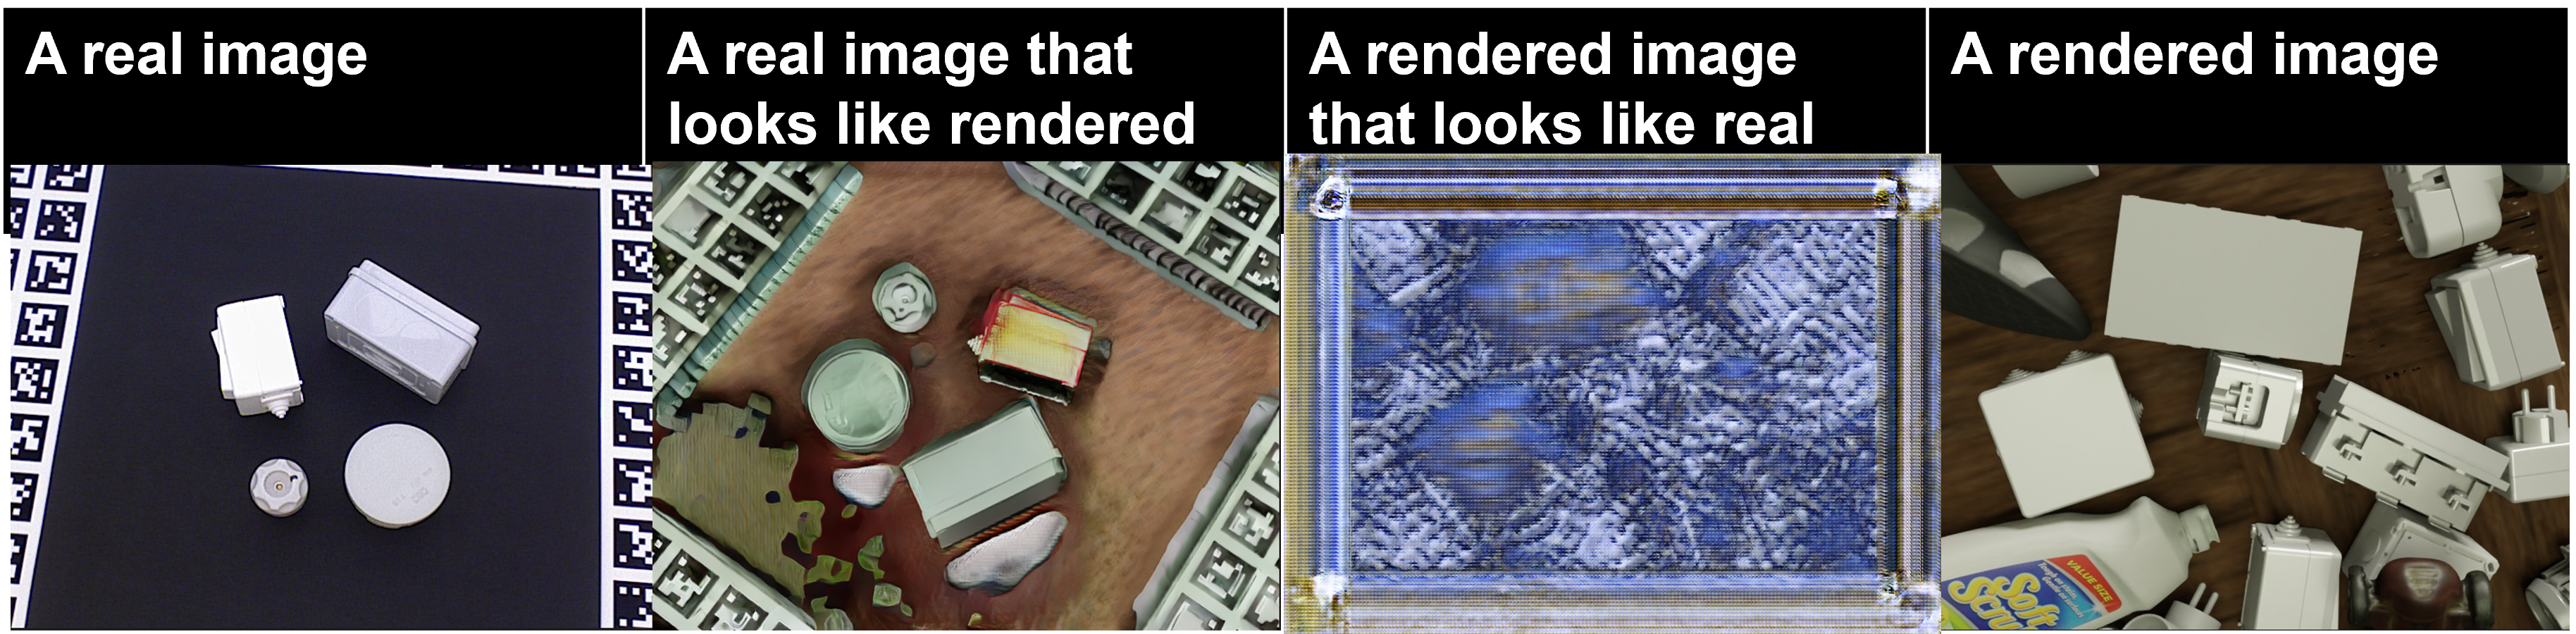
\includegraphics[width=14cm]{./cyclegan.png}
	\end{center}
	\begin{center}
		\label{cyclegan}
	\end{center}
\end{table}

As it can be noted, even after an extensive training with a massive dataset of nearly 50 000 images, Cycle-GAN still produced fairly low-quality results, especially for the real-alike images. This problem has also been acknowledged by Zhu et al. as a limitation of Cycle-GAN \cite{Zhu2017}, where differences in the distribution characteristics of the training dataset caused similar artifacts. Due to the low performance on the T-LESS dataset and long training time, this method was excluded from further tests. 

\FloatBarrier

\subsection{Experiments with Adaptive Teacher}
\label{ensemExp} 
For the next set of experiments, this thesis proposes to analyze an ensembled setup. An ensembled setup is a combination of multiple algorithms that leverage their benefits to produce a superior result. In regards to domain-adaptive object detection, such setups were summarized earlier in the \nameref{mean_teacher} section. As a base study for this thesis, the Adaptive Teacher \cite{Li2021} model is studied extensively. Unlike the architectures in the previous experiments, mean teacher training frameworks implement multiple adaptation strategies. In case of the Adaptive Teacher method, Li et al. proposed to use both adversarial and pseudo-labeling techniques that are embedded into the student-teacher framework. 

To validate the suitability of this architecture, the code base has been modified to utilize the prepared T-LESS dataset and was trained as-it-is. Figure \ref{adapt_experiment1} illustrates the results of the visualization after training such model. Similarly, to the previous experiments, the model was based on Faster-RCNN \cite{ima} and a ResNet \cite{He2015} backbone network with 101 layers, which was pre-trained on the ImageNet  \cite{Russakovsky2014} dataset. Although traditional ML and DL algorithms utilize the term epoch, which stands for one forward and one backward passes of the loop for the entire set of the training samples, in Detectron2 \cite{wu2019Detectron2} the term "iterations" is used instead. Iterations denote a number of times to complete the forward and backward passes for a batch of training samples, where a batch is a small subset of data. 

\begin{figure}[htb]
    \centering
    \subfloat[Visualization on the source dataset]{{\includegraphics[width=6cm]{./experiments_original_1.png} }}%
    \qquad
    \subfloat[Visualization on the target dataset]{{\includegraphics[width=6cm]{./experiments_original_2.png} }}%
    \caption{Results of the experiments with Adaptive Teacher as it is.}\label{adapt_experiment1}%
\end{figure}

Naturally, the model performed poorly on the custom dataset without tweaking any hyperparameters. Although the performance on the source dataset is more than satisfactory (Figure \ref{adapt_experiment1} (a)), random artifacts take place in the form of noisy bounding boxes, as can be seen in Figure \ref{adapt_experiment1} (b). For this round of experiments, the number of iterations was set as high as possible in order to explore the limits of the setup. Although the model was trained for 360 000 iterations, such huge values are often redundant as the selected dataset has extensive amount of images and, thus, less iterations can be used, as will be presented in \nameref{results}. 
\todo{perhaps convert iterations to epochs} 

To overcome the issue of noisy predictions, two steps have been carried out. First, the LR scheduler has been adjusted in the original Adaptive Teacher \cite{Li2021} implementation. In the original setup, the Adaptive Teacher algorithm used a warm-up two-stage multi-step scheduler. This scheduler initializes the LR in two stages.  First gradually increases for a duration of warm-up $\texttt{WARMUP\textunderscore ITERS} = 1000$ iterations, until it reaches the fixed $\texttt{BASE\textunderscore LR} = 0.001$.  Instead, this thesis suggests to use a multi-stage cosine-annealing scheduler without restarts, as suggested by Loshchilov et al. \cite{Loshchilov2016}. In these experiments, the learning rate first slowly ascends to the $\texttt{BASE\textunderscore LR} = 0.001$. However, as the ceiling is reached, it starts to decay to zero by the time of the last iteration $\texttt{MAX\textunderscore ITERS}$ is reached. This in theory allows to protect the scheduler from overshooting as it approaches the global minimum. Although Loshchilov et al. additionally proposes resetting the scheduler after it reaches the minimum, in this thesis such implementation is neglected for the time being. Both schedulers are compared against each other and are illustrated in Figure \ref{annealing}.

Another issue that potentially caused the noisy predictions on the real images is over-fitting. This might happen when, given the model complexity, the model is trained for an excessive amount of time. As a result, the model would only perform well on the training data. 
Therefore, in order to identify the suitable number of iterations required for training, an early stoppage algorithm was added. Instead of checking whether the loss keeps decreasing, the \texttt{AP50} metrics is tracked for the validation set at every $\texttt{EVAL\textunderscore PERIOD} = 1000$ interval. The best \texttt{AP50} value is stored for the total of $\texttt{PATIENCE} = 10$ times. If the value does not improve for longer than $\texttt{EVAL\textunderscore PERIOD} \times \texttt{PATIENCE}$ iterations, the best model is saved and the training is terminated. Otherwise, the new best \texttt{AP50} is recorded. The results of such modification are presented later in the \nameref{results} section.  

\begin{figure}[htb]
	\begin{center}
		\includegraphics[width=14cm]{./LR.jpg}
	\end{center}
	\caption{a) The original LR scheduler against b) The proposed cosine annealing LR scheduler without restarts.}
	\begin{center}
		\label{annealing}
	\end{center}
\end{figure}
\FloatBarrier

\subsection{Regularized Cross-Domain Adaptive Teacher}
\label{mainExperiments} 
In the subsequent sections, a novel architecture will be introduced. The effectiveness of the existing methods has been evaluated to address domain shift  between various open-source datasets. Most often domain adaptation is performed to transfer knowledge from one dataset for autonomous driving(Cityscapes) to another(Foggy-Cityscapes, Sim10k, KITTI), or to transfer knowledge from one dataset with general objects (PASCAL VOC) to another(Clipart, Watercolor, Clipart) \cite{Oza2021}.  

However, no comprehensive work have addressed the industrial cross-domain object detection. Additionally, motivated by works of Li et al. \cite{Li2021} and Xu et al. \cite{Xu2020}, this thesis assesses the practicality of the categorical regularization in the Adaptive Teacher framework. Unlike the original architecture of Adaptive Teacher \cite{Li2021}, the model is aligned at two stages:  image-level and instance-level. Following Chen et al. \cite{Chen2018} and Xu et al. \cite{Xu2020}, a consistency loss term has been added to regularize both stages. The training process follows similar principles to the ones outlined in the \nameref{ensemExp} section. The proposed architecture is presented in Figure \ref{mymodel}. 

\begin{figure}[htb]
	\begin{center}
		\includegraphics[width=16cm]{./MyModel.png}
	\end{center}
	\caption{A proposed architecture for cross-domain object detection. Blue elements represent standard Faster-RCNN components, purple elements - domain adaptation components and yellow elements are Faster-RCNN modified components for continual learning, which will be discussed later.}
	\begin{center}
		\label{mymodel}
	\end{center}
\end{figure}

Chen et al. \cite{Chen2018} proposed one of the first methods to use a two-level alignment, which was discussed earlier in the \nameref{adv_approach} section. Xu et al. \cite{Xu2020} expanded further on this method by adding a consistency regularizing term. Upon analyzing multiple papers, Xu et al. comments that using only image-level adaptation would result in the alignment of the non-transferable background regions between the source and target domains, which would in turn result in poor accuracy in the target domain \cite{Xu2020}. Instance-level alignment would allow to reduce the distance between the local features, such as object appearance, size and viewpoint \cite{Chen2018}. On the other hand, it is not possible to omit image-level alignment as it is important to address adaptation of the global features of the image, such as image scales, illumination and style \cite{Chen2018}. 

Therefore, this setup employs a mean teacher based Faster-RCNN \cite{ima} setup with two domain adaptation networks in the student model. Similarly to the preceding architectures \cite{Li2021,Liu2021}, data augmentation is used to assist in the training process, For these experiments, random cropping was excluded from tests as it was negatively affecting the pseudo-labeling. Instead, a few other transformations such as histogram equalizing and sharpness adjustments, were added to the strong augmentations list. The complete list of used augmentations is shown in Figure \ref{newAugmentations}. It is believed that random rotations and affine transformations are not as important with the T-LESS dataset as the number of images taken in a rotational manner seems to be fairly sufficient.

\begin{figure}[htb]
	\begin{center}
		\includegraphics[width=16cm]{./Tless_augm.png}
	\end{center}
    \caption{Augmentations used in the experiments.}
	\begin{center}
		\label{newAugmentations}
	\end{center}
\end{figure}

Identically to the earlier experiments, the backbone was chosen to be ResNet \cite{He2015} with 101 layers. Following Li et al. \cite{Li2021}, one adaptation module is attached to the output of a CNN backbone.  Another domain adaptation network is attached to the output layers of Faster-RCNN. While the backbone generates image-level features, output layers of Faster-RCNN produce the foreground region proposals. Both modules utilize a standard GRL block \cite{Ganin2015} followed by a domain classifier.


In this work, the image-level domain classifier is similar to the basic CNN architecture illustrated in Figure \ref{CNN} and it was defined in accordance with the setup of Li et al. \cite{Li2021}. It has three convolutional layers with batch normalization and leaky-ReLUs followed by a convolutional classier layer. The instance-level classifier resembles the architecture in \cite{Xu2020} and consists of two linear layers with leaky-ReLUs and dropout layers and finalized with a classifier and a sigmoid. Dropout layers were added due to the reasons specified in Section \ref{alexnet_section}. A detailed description of the architecture can be found in the \nameref{appendix}. 

Naturally, both an image and a region proposed by Faster-RCNN should represent the same domain. Similarly to Xu et al., to minimize the difference between predictions of the domain classifiers, they are regularized using $\mathcal{L}_{\text {consist }}$ consistency loss. In these experiments, consistency loss is based on simple MSE loss between instance- and image-level domain classifier loss terms $\mathcal{L}_{\text {ins }}$ and $\mathcal{L}_{\text {img }}$, as it was described in Equation \ref{MSE_eq}.

The calculations of both $\mathcal{L}_{\text {ins }}$ and $\mathcal{L}_{\text {img}}$ follow the practices outlined in Equation \ref{faster_DA_losses}. Additionally,  the consistency loss $\mathcal{L}_{\text {consist }}$ follows the formula in Equation \ref{faster_DA_losses_consist}. However, instead of L2 norm, MSE is utilized.  

To trade-off between different loss parameters, the weights of the domain classification and consistency losses have been added to the original setup of the Adaptive Teacher network. The complete formula for loss computation is displayed in Equation \ref{total_loss}. 

\begin{equation}
\mathcal{L}=\mathcal{L}_{\text {sup }}+\lambda_{\text {unsup }} \cdot \mathcal{L}_{\text {unsup }}+\lambda_{\text {img }} \cdot \mathcal{L}_{\text {img }}+\lambda_{\text {ins }} \cdot \mathcal{L}_{\text {ins }}+\lambda_{\text {consist }} \cdot \mathcal{L}_{\text {consist }},
\label{total_loss} 
\end{equation}

where $\mathcal{L}_{\text {sup }}$ is the standard Faster-RCNN detector loss in the student model; $\mathcal{L}_{\text {unsup }}$ is the unsupervised loss between pseudo-labels generated by the teacher model and supervised predictions and the $\lambda$-s are the corresponding hyper-parameters to trade-off the weights of different loss terms. The $\mathcal{L}_{\text {sup }}$ is calculated in a similar manner as it was introduced earlier in Equation \ref{faster_rcnn_loss}. 
 
Pseudo-labels for the unlabeled target dataset are obtained identically as in the original Adaptive teacher implementation \cite{Li2021}. The noisy pseudo-labels are filtered using a confidence threshold and a class-wise NMS \cite{Liu2021}. These pseudo-labels are used as ground-truth in the calculation of the unsupervised loss $\mathcal{L}_{\text {unsup }}$. The unsupervised loss is essentially based on a standard Faster-RCNN loss. However, it does not include the bounding box regression loss, as it not possible to filter out the bounding boxes using only confidence threshold, which was defined   by Liu et al. \cite{Liu2021}.  Instead, to improve the quality of pseudo-labels, EMA is applied to gradually move weights from the student to the teacher model as discussed in the  \nameref{mean_teacher} section, and it is the only place where updating the teacher model takes place \cite{Li2021}.  
 
Multiple experiments have been conducted with the architecture defined in Figure \ref{mymodel}. These experiments will be discussed in the \nameref{results} section. In the following section, a proposed continuously learning domain-adaptive object detection setup is introduced. 

\FloatBarrier

\subsection{Object detection with continual learning}
\label{cont_learning_section} 
Although the pre-trained model performs fairly well on the target dataset, it will not be able to predict unknown objects. In order to solve the scalability problem defined in the \nameref{objective}, the proposed architecture should be able to keep learning when new data is added. Often such problems are addressed by a special case of transfer learning known as "fine-tuning". A typical example of fine-tuning is done by retraining the top level components of the network. This procedure would enable the network to apply previously learned knowledge on an unknown yet similar problem, while significantly reducing the training time. In regards to the objectives of this thesis, it would allow to utilize the knowledge of the previously learned equipment parts to promptly retrain it and apply it to new classes of objects. 
In the first set of experiments, a naive fine-tuning approach was attempted. The model was trained based on the architecture, which was demonstated in the \nameref{mainExperiments}. The regular training stage included both source and target datasets that contained classes 1 to 20, while the fine-tuning stage only included the data for classes 21-30 and the pre-trained weights file from the previous stage. After the model has been trained on the first 20 classes, the FC layers of the trained model have been removed and replaced with new FC layers that can produce predictions for 30 classes. Both models were trained for the same number of iterations. The results are presented in Table \ref{naive_finetuning}.

\begin{table}[htb]
\caption{The naive fine-tuning results.}
\label{naive_finetuning}
\resizebox{\textwidth}{!}{%
\begin{tabular}{l|l|l|ll}
\cline{2-3}
                                         & Model trained on data from classes 1-20      & Model trained on data from classes 21-30   &  &  \\ \cline{1-3}
\multicolumn{1}{|l|}{Base learning rate} & 0.001                              & 0.0005                           &  &  \\ \cline{1-3}
\multicolumn{1}{|l|}{Outputs}            & Predictions for 20 classes         & Predictions for 30 classes       &  &  \\ \cline{1-3}
\multicolumn{1}{|l|}{Max iterations}     & 35000                              & 35000                            &  &  \\ \cline{1-3}
\multicolumn{1}{|l|}{Training time}      & about 8 hours                      & about 8 hours                    &  &  \\ \cline{1-3}
\multicolumn{1}{|l|}{Data} &
  \begin{tabular}[c]{@{}l@{}}source (labeled) and target (unlabeled) \\ datasets limited to classes 1-20\end{tabular} &
  \begin{tabular}[c]{@{}l@{}}Saved weights(.pth) from the original model(1-20) \\ + datasets limited to classes 21-30\end{tabular} &
   &
   \\ \cline{1-3}
\multicolumn{1}{|l|}{Results}            & \textbf{AP} 58.1596, \textbf{AP50} 75.27, \textbf{AP75} 66.89 & \textbf{AP} 19.93, \textbf{AP50} 29.78, \textbf{AP75} 22.36 &  &  \\ \cline{1-3}
\end{tabular}%
}
\end{table}

As can be easily noted, the results dropped significantly even though the initial weights are supposed to give a decent advantage at the start. This setup would not only have low performance on the new data, but also unable to classify and localize original dataset. A few important modifications were considered in the next experiment: 

\begin{enumerate}
\item In order to fine-tune the network successfully, a freezing process should be carried out on the deeper, more specifically, on the backbone layers of the network. Skipping this step is the main result of the performance drop in Table \ref{naive_finetuning}. By freezing deeper parts of the network, key trained features will be preserved, and the number of trainable parameters will be reduced, which will in turn speed up the training time. 
\item Too many unfamiliar cases will lead to a higher performance drop. Adding fewer additional classes in each subsequent task will help to maintain the performance drop at the lower level. This has been proven by experiments of Peng et al. \cite{Peng2020}. In other words, instead of retraining the original model with 10 more unknown classes, the model should be retrained with one or two at most. 
\item Additionally, the weights file \texttt{.pth}, which was originally trained for the first $N$ classes, also contained the states of the optimizer, i.e. of the training process. This included the iteration number and the learning rate at that iteration. As a result, the training process is started from a much lower base LR, thus decreasing the training speed. Therefore, before proceeding further, the optimizer states were removed from the dictionary of the weights file. 
\item Finally, instead of replacing the original FC layers altogether, a new architecture is proposed, as illustrated in Figure \ref{continualModel} (b). 
\end{enumerate}

Following the studies presented in the \nameref{cont_learning} section, the detector head of the custom model is additionally modified to address a scalable training setup. The architecture presented in Figure \ref{continualModel} (b) replicates the method proposed by Rusu et al. \cite{Rusu2016}, but applies it in a cross-domain mean teacher setup. An overview of this method was shown earlier in Figure \ref{mymodel}, where both detector heads of the student and the teacher networks are modified. In this experiment, the original detector head is frozen, which includes both the classifier and the box regressor. Freezing essentially prevents the weights from being modified by disabling the learning rate updates. Consequently, new output layers are attached to the network. These layers are responsible for the unknown $M$ number of classes and unlike the original detector, they are not frozen. The original detector head classifies an $N+1$ number of objects, which also includes the background. Therefore, to preserve data integrity, the appended detector head ignores the background class and only predicts $M$ new objects. 

One potential disadvantage to such approach is that the original detector head is trained to recognize the background as well, which also included the shapes of the new $M$ objects. Moreover, the weights for the original detector are frozen. Therefore, it is believed that the appended detector head will struggle predict the new classes if the original detector forces it to be predicted as "background". 

To solve this problem, a new architecture has been introduced in Figure \ref{continualModel} (c). This model further combines the ideas proposed by Rusu et al. \cite{Rusu2016} and Donahue et al. \cite{Donahue2013}, which were introduced in the \nameref{cont_learning} section. Instead of completely freezing the original detector weights, the learning rate is regularized by reducing the base learning rate for the previously trained classifier. The extended FC layers are trained with a standard LR.  According to Parisi et al. \cite{Parisi2018}, reduced learning rate will prevent the model from making significant changes in the original weights, while also learning new data. This might potentially enable the network to slowly be re-trained and learn the difference between the new classes and the background. Meanwhile, the dynamically expanding architecture of Rusu et al. \cite{Rusu2016} will focus on fighting the catastrophic forgetting problem. Ultimately, in the proposed method the model aims to learn new data using network expansion with regularization. The results of implementing such architecture are summarized in the \nameref{cont_learning_results} section. 


\begin{figure}[htb]
	\begin{center}
		\includegraphics[width=16cm]{./FC.png}
	\end{center}
	\caption{A proposed architecture for continual learning setup. Blue elements represent standard Faster-RCNN components, yellow elements are modified components for continual learning.}
	\begin{center}
		\label{continualModel}
	\end{center}
\end{figure}
\FloatBarrier


\clearpage